\documentclass{standalone}
\usepackage{pgfplots}
\pgfplotsset{compat=1.18}
\begin{document}
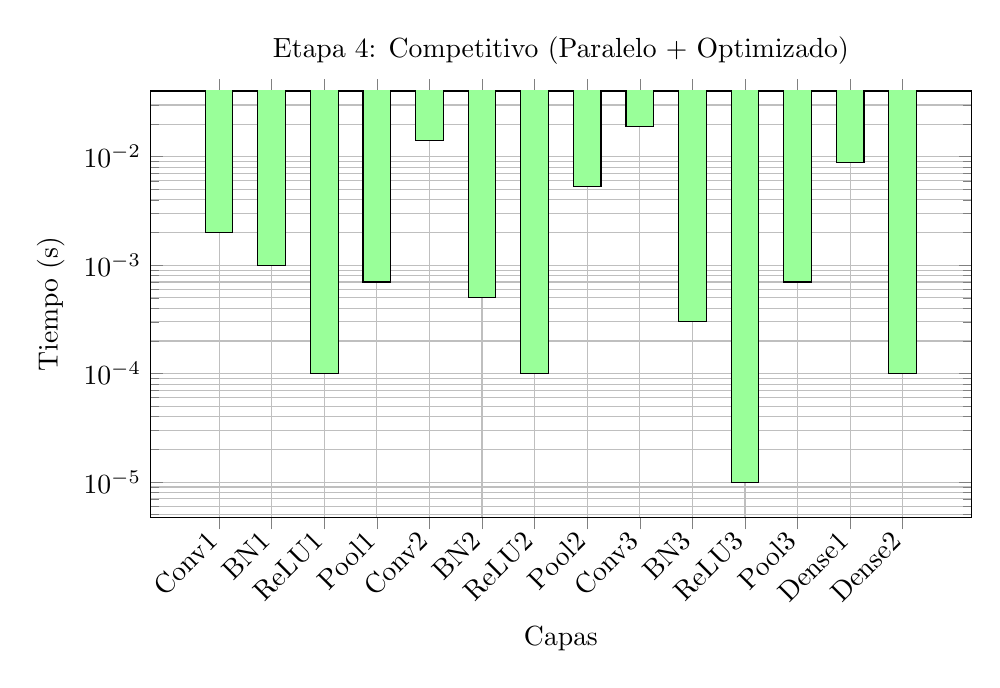
\begin{tikzpicture}
\begin{axis}[
    ybar, ymode=log, width=12cm, height=7cm,
    ylabel={Tiempo (s)}, xlabel={Capas},
    xtick=data, xticklabels={Conv1, BN1, ReLU1, Pool1, Conv2, BN2, ReLU2, Pool2, Conv3, BN3, ReLU3, Pool3, Dense1, Dense2},
    x tick label style={rotate=45, anchor=east},
    title={Etapa 4: Competitivo (Paralelo + Optimizado)},
    grid=both
]
\addplot[fill=green!40] coordinates {
    (1,0.0020) (2,0.0010) (3,0.0001) (4,0.0007) 
    (5,0.0141) (6,0.0005) (7,0.0001) (8,0.0053) 
    (9,0.0190) (10,0.0003) (11,0.00001) (12,0.0007) 
    (13,0.0089) (14,0.0001)
};
\end{axis}
\end{tikzpicture}
\end{document}
